\documentclass{beamer}
\usetheme{Boadilla}
\usepackage{essay-def}
\usepackage{bm}
\usepackage{amsfonts}
\usepackage{amssymb}
\usepackage{amsmath}
\usepackage{amsthm}
\usepackage{comment}
\usepackage{geometry}
\geometry{left=1cm,right=1cm}
    \title[Distribution Mismatch]{Combatting distribution shift in SciML}
\author[J. Zhao]{Jiaxi Zhao}
\date{20th Mar, 2024}
\begin{document}
\par \setlength{\parindent}{2em}

\begin{frame}
\titlepage

\end{frame}

\begin{frame}{An abstraction of SciML workflow}
	Simulating the dynamics:
	\bequn
		\begin{aligned}
			\mathbf{0} & = \mcL(\mfx, \p_t \mfx, \mfu, t), \quad \mfx \in \mcX, \mfu \in \mcU, \mcL: \mcX \times T\mcX \times \mcU \times \mbR_+ \rightarrow \mbR^{c},			\\
			\mfu & = \phi(\mfx, t), \quad \phi: \mcX \times \mbR_+ \rightarrow \mfu.
		\end{aligned}
	\eequn
	\begin{itemize}
		\item 1. $\mcL$ is known, possibly non-linear.
		\item 2. $\phi$ is un-known.
		\item 3. A set of data pairs $\lbb (\mfx_1, \mfu_1, t_1), (\mfx_2, \mfu_2, t_2), \cdots, (\mfx_N, \mfu_N, t_N )\rbb. $
		\item 4. Benchmark algorithm solves the ordinary least square:
		\bequn
			\arg\min_{\theta} \mbE \norml \mfu - \phi_{\theta}(\mfx, t) \normr^2.
		\eequn
	\end{itemize}

\end{frame}

\begin{frame}{Iterative scheme is ubiquitous}
	There are different levels of iterative methods in scientific application:
	\begin{itemize}
		\item 1. High level: iterative method for forward and inverse problem
			\begin{itemize}
				\item * Steady simulation: RANS.
				\item * Unsteady simulation: LES, Molecular dynamics.
				\item * Optimization for inverse problem: inverse scattering.
			\end{itemize}
		\item 2. Low level: iterative method to solve the linear system:
			\begin{itemize}
				\item * Jacobi, Gauss-Seidel, SOR etc.
				\item * Connjugate gradient, GMRES, BiCGSTAB etc.
				\item * Preconditioning, e.g. ILU, AMG etc.
			\end{itemize}
	\end{itemize}
\end{frame}

\begin{frame}{Dilemma of data-driven scientific computing}
	In the data-driven scientific computing, \textcolor{red}{\textbf{dynamics structure}} can cause \textcolor{red}{\textbf{distribution mismatch}} between the training and testing data.
	\begin{figure}[H]
          \centering
          \centerline{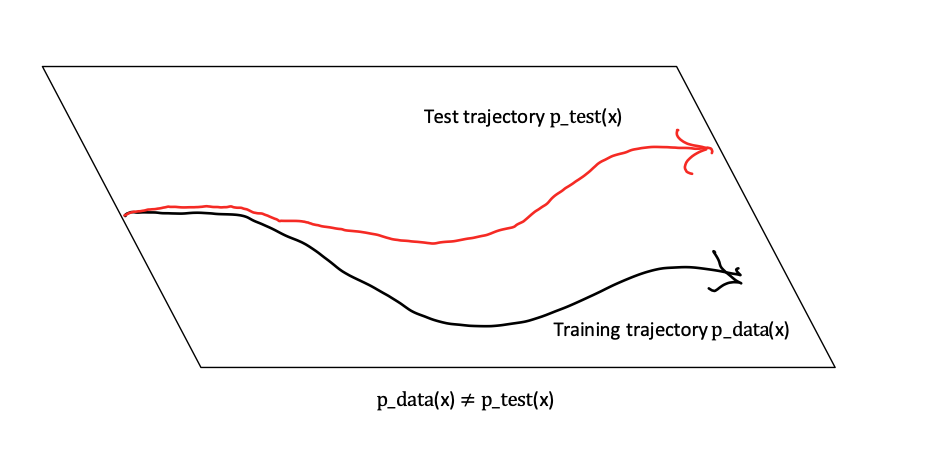
\includegraphics[width=\linewidth]{fig/dilemma.png}}
        \end{figure}
\end{frame}

\begin{frame}
	\begin{itemize}
		\item \textbf{Data generation:}
		\begin{itemize}
			\item Preprocessing, e.g. filterd DNS data compared with LES data
			\item Adaptive sampling \& Active learning
			\item Importance reweighting
		\end{itemize}
		\item \textbf{Learning algorithm:}
		\begin{itemize}
			\item Manifold-regularized learning
			\item Unrolled dynamics and reinforcement learning
		\end{itemize}
		\item \textbf{Simulated algorithm:}
		\begin{itemize}
			\item Subspace-aware algorithm
			\item Random subspace method
		\end{itemize}
	\end{itemize}
\end{frame}

\begin{frame}{Manifold regularization}
	Regularization encodes the information of the data manifold.
	\begin{figure}[H]
		\centering
		\centerline{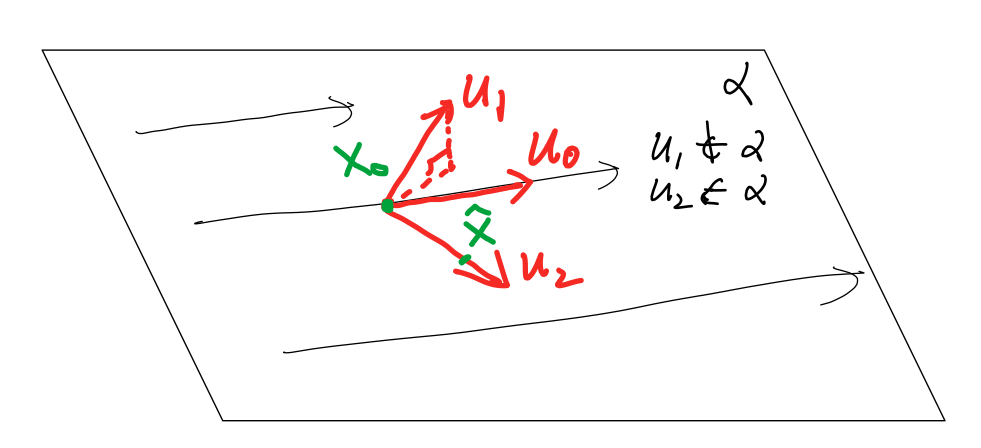
\includegraphics[width=0.9\linewidth]{fig/mfd.png}}
	\end{figure}
\end{frame}

\begin{frame}{The freedom of choosing simulated dynamics}
	For unsteady simulation problem, we can change the numerical scheme for simulation, i.e.
	spatial and temporal discretization. While for steady state simulation and inverse problem, we can 
	choose or design the numerical scheme:
	\begin{equation}
		\begin{aligned}
			\mathbf{0} & \ = \mcL_{\theta}(\mfu),	\\
		  \p_t \mfu & \ = \mcL_{\theta}(\mfu), \quad \text{(RANS simulation)}   \\
		  \p_t \mfu & \ = - \lp \nabla_u\mcL_{\theta}(\mfu) \rp^{-1} \mcL_{\theta}(\mfu) \quad \text{(Gauss Newton)}.
		\end{aligned}
	\end{equation}  
	The question is: \textit{How to go beyond linear?}
\end{frame}

\begin{frame}{Generative SGS modeling}
	
\end{frame}



\begin{frame}{Code development}
	Develop a codebase to implement different algorithm for improving the stability
	of the hybrid solver, e.g. regularization-based method, active-leraning method, etc.

	\url{https://github.com/jiaxi98/ml4dynamics}

	Data-driven turbulence modeling platform based on OpenFOAM
	\url{https://github.com/jiaxi98/pyfoam}
\end{frame}

\end{document}